\section{Quantifying Baryon Redistribution}
\label{sec:feedbackmetrics}

Feedback is a complex process that impacts a wide range of baryonic
observables, from the galaxy stellar mass function, to galaxy sizes, to the
density profiles of galaxies \citep[e.g.][]{Angles-Alcazar2014, Nelson2015,
Hellwing2016, BenitezLlambay2018}. It is interesting, therefore, to develop
tools to study the global effects of feedback directly, as a complement to
the many indirect constraints obtainable from comparing to astrophysical
observables. Here we describe the {\it spread metric} as a general tool to
examine the redistribution of baryons via feedback relative to the underlying
dark matter distribution.

\subsection{The Spread Metric}

\begin{figure}
    \centering
    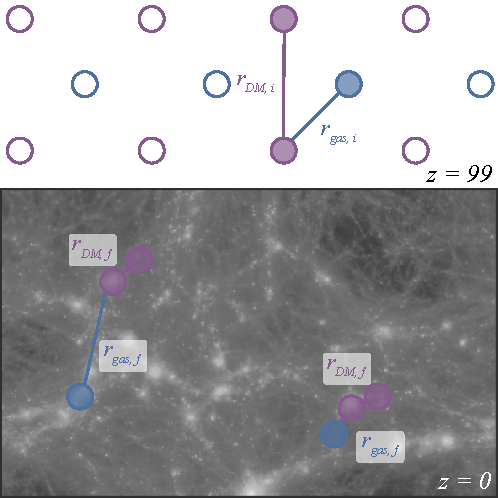
\includegraphics[width=\columnwidth]{figures/kspafig_small.pdf}
    \vspace{-0.5cm}
    \caption{Illustration of the matching procedure between initial and final
    conditions to define the spread metric. Gas particles are shown in
    purple, with dark matter particles shown in blue. The top panel shows the
    $z=99$ initial conditions, where every particle finds its nearest dark
    matter neighbour. The bottom panel shows the distances between those
    particles at $z=0$. For our fiducial results, each particle is matched to
    the three nearest neighbours at $z=99$ and the spread metric is computed
    as the median of the corresponding distances at $z=0$ (see text for
    details).}
    \vspace{-0.5cm}
    \label{fig:kspafigsmall}
\end{figure}

Our approach to quantifying the large-scale impact of feedback is to develop
a simple and robust metric that directly captures the displacement of gas
owing to feedback. This {\it spread metric}, illustrated in Fig.
\ref{fig:kspafigsmall}, works as follows:

\begin{enumerate} 
	\item For every gas particle $i$ in the initial conditions, find the nearest
          $n$ dark matter neighbours $j$ (with $n=3$ for our fiducial results).
	\item In the final conditions at $z=0$, match all remaining baryonic particles
	      with their initial conditions progenitor (in this case, stars are
	      matched with their gas particle progenitor).
    \item Find the distance $r_{ij}$ between particles $i$ and $j$ in the
          final conditions
    \item The spread metric for particle $i$, denoted $S_{i}$, is given by the \emph{median}
          of the $n$ original dark matter neighbour distances $r_{ij}$.
\end{enumerate}

\begin{figure}
    \centering
    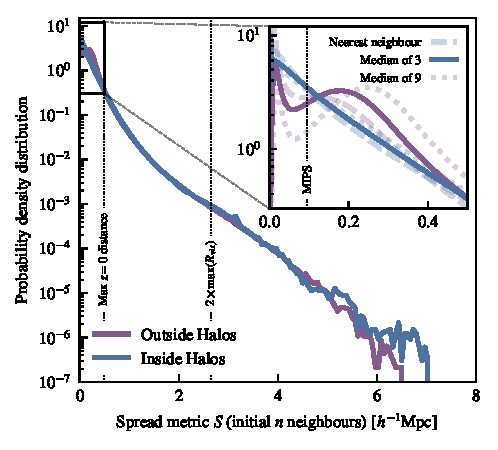
\includegraphics{figures/s50j7kAHF/dark_matter_distance_figure_s50j7k_AHF}
    \vspace{-0.5cm}
    \caption{The redshift $z=0$ spread metric distribution for the dark
    matter component in the full \simba{} model. The distribution is split
    between particles that lie within haloes (blue) and outside haloes
    (purple), with this being an approximately even split at $z=0$. Vertical
    dotted lines indicate the maximal distance between any two nearest dark
    matter particles at $z=0$ ($\sim 0.5\hmpc{}$) and twice the maximal
    virial radius of any halo in the box (${\rm max}(R_{\rm vir}) \sim
    1.3\hmpc{}$). The inset figure shows the inner $0.5\hmpc{}$ of the
    distribution, with the mean inter-particle separation in the initial
    conditions (MIPS $\sim 0.1\hmpc$) indicated by the vertical dotted line.
    The fainter lines show how the spread metric changes when taking the
    median over a different number of initial nearest neighbours.
    This figure shows that initially neighbouring dark matter particles
    can be spread out to $7\hmpc{}$ owing to gravitational dynamics alone.}
    \vspace{-0.5cm}
    \label{fig:dmonlyspread}
\end{figure}


The spread metric is introduced to measure the net displacement of baryons over
cosmic time. This is somewhat difficult to do in practice, as to measure the
net movement of particles we require a reference point. We take that
reference point to be the initially neighbouring dark matter particle as to
respect the Lagrangian nature of the simulation. This is different to taking the
relative motion of the particle compared to its initial point in co-moving space
as it ensures that there is zero `spread' in bulk motions.

The spread metric is presented first for dark matter in Fig.
\ref{fig:dmonlyspread}, showing the probability density distribution of the
spread $S$ for dark matter particles either inside (blue) or outside (purple)
of virialized haloes at $z=0$. This quantifies the redistribution of the dark
matter due to any gravitational effects (note that back-reaction effects from
the gas dynamics are not seen in the spread metric). We see here that the
largest spread distances are significantly larger than any of the
characteristic distances; this is even compared to the largest separation for
any two particles at $z=0$, implying that these distances are much further
than can be achieved from Hubble expansion in voids alone. The overall
distribution follows an exponential decay, with exponentially fewer particles
(once outside the inner $\sim 0.5 \hmpc{}$) being found at larger distances.
There are many possible explanations for these results, from tidal stripping
of objects that end up never merging, accretion of dark matter from
satellites \citep[see e.g. the effects in ][]{VandenBosch2018}, or even
particles on randomised orbits from recently accreted material that end up on
opposite sides of the `splashback' region \citep{Diemer2014, Adhikari2014}.
This splashback region is sometimes larger than the virial radius of the
halo, meaning that two particles may be separated by up to $4R_{\rm vir}$
through this process \citep{Diemer2017a}. In practice, we expect the final
distribution to be a mixture of the three, with other as-of-yet unknown
effects also contributing.

In Fig. \ref{fig:dmonlyspread} we also show the consequences of choosing to
average over different numbers of initial neighbours. The simplest metric
would use a single nearest neighbour in the initial conditions, rather than
the median over $n$ initial neighbours. The choice of $n=3$ was made
primarily to ensure that the dark matter results were robust when comparing
matter inside and outside of haloes. For a given dark matter particle pairing,
a large distance between two neighbours would be `double counted' for the
case where one neighbour makes it into a halo and one remains outside,
contributing the large distances to both bins. Choosing $n=3$ enables the
median result to represent the distance to a real particle, and removes the
problem of double counting for the nearest neighbour. The overall
distributions of distances were not changed much by this choice, however
larger choices for $n$ increase the contrast in the dark matter images in
Fig. \ref{fig:bigdistanceimage}, with more substructure picked up in the
low-spread particles, and show more diffuse structure in the high-spread
particles.

\subsection{Baryon Spreading in \simba{}}

Fig. \ref{fig:distbaryon} shows how the distribution of spread distances
for the gas particles is significantly different to that for the dark matter.
Gas particles are able to spread to much larger distances, up to $12\hmpc{}$
(approximately 10 times the virial radius of the largest halo in the box!),
compared to the $7\hmpc{}$ that dark matter can reach. We also see that even
gas inside of haloes at $z=0$ has spread significantly more than the dark
matter when explicitly selecting for this component. This suggests a
different origin for the gas and dark matter content of haloes.

Another interesting component is the gas that originated in Lagrangian
regions (i.e. next to the dark matter that will reside in haloes at $z=0$),
indicated by the blue dashed line. With the baryon fraction of haloes being
typically less than $50\%$ of the cosmic mean, we should expect that a
significant amount of Lagrangian gas is lost over time, possibly spreading to
large distances out of haloes owing to high energy feedback events, either
through galactic winds or AGN feedback. In \simba{}, we see that gas from
Lagrangian regions indeed spreads systematically further, with a factor of
$\sim 2$ more particles at distances larger than $\sim 4 \hmpc{}$ than an
unbiased selection would suggest.

\begin{figure}
    \centering
    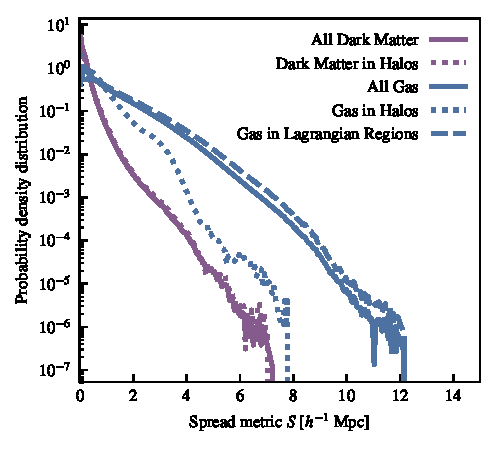
\includegraphics{figures/s50j7kAHF/distance_plot_split_by_component+AHF.pdf}
    \vspace{-0.5cm}
    \caption{Spread distance distribution for gas at $z=0$ (blue) compared to
    that of the dark matter component (purple). Solid lines indicate the full
    distribution, dotted lines correspond to matter inside $z=0$ haloes, and
    the blue dashed line shows the distribution for gas that was inside of
    Lagrangian regions at $z=99$. The distributions for gas inside haloes and
    outside haloes are significantly different, with gas that resides outside
    haloes being preferentially spread to larger distances than gas on
    average. Note that only 10\% of the gas in the entire simulation is in
    haloes at $z=0$. Gas that originated in Lagrangian regions is
    preferentially spread the most, with a factor of 2 offset over the
    unbiased selection at large spread distances.}
    \vspace{-0.5cm}
    \label{fig:distbaryon}
\end{figure}

\begin{figure*}
    \centering
    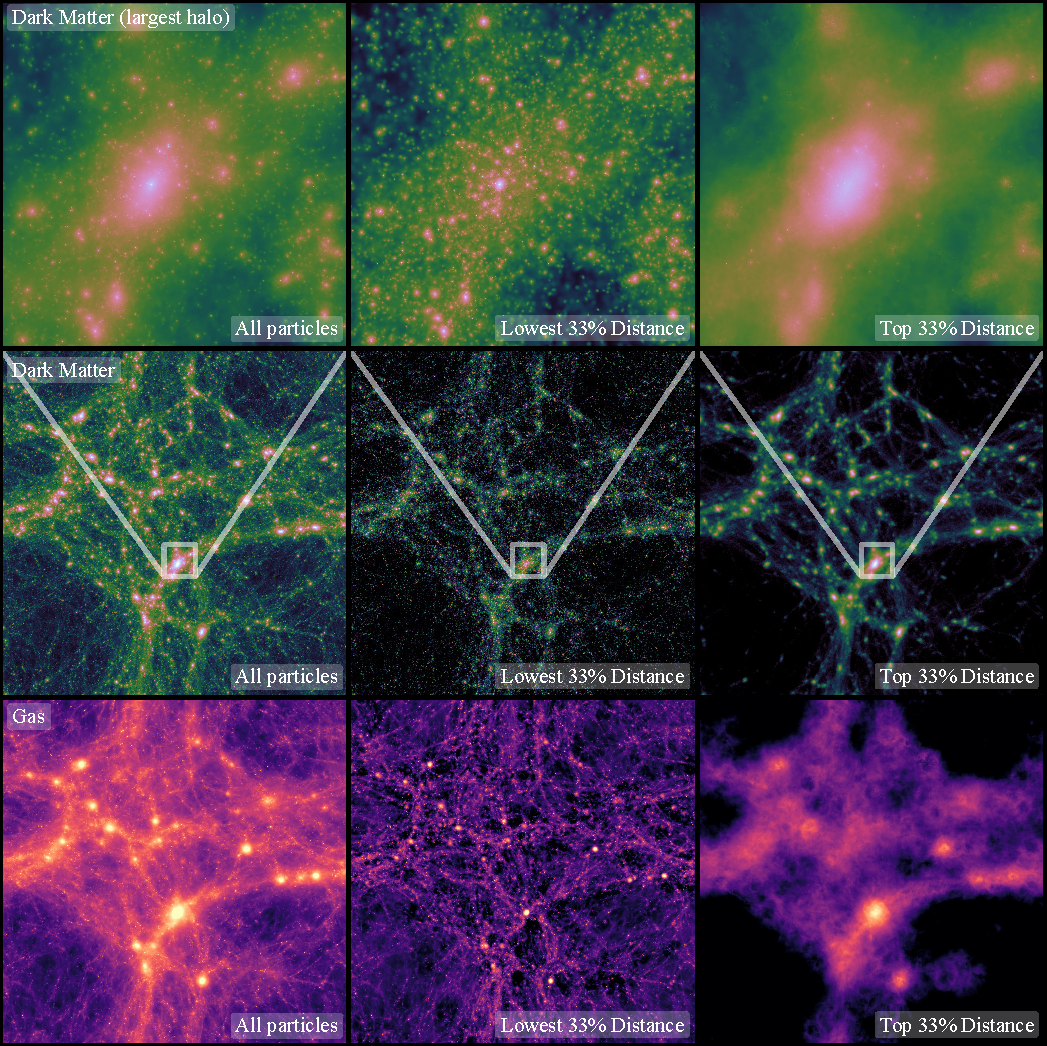
\includegraphics[width=\textwidth]{figures/distance_figures_3.pdf}
    \caption{Projected mass surface density distributions for different
    particle selections at $z=0$. The three rows show, from top to bottom,
    the dark matter in a $4.5\hmpc{}$ cubic volume centred around the largest
    halo ($R_{\rm vir}\sim 1.3\hmpc{}$) and the dark matter and gas
    distributions in the $50\hmpc{}$ box. Columns show, from left to right,
    all particles inside of the corresponding volume, the 33\% of the
    particles with the lowest spread distance, and the 33\% of the particles
    that have spread the most. For the dark matter, these cuts correspond to
    particles that have travelled less than $0.1\hmpc{}$ and more than
    $0.25\hmpc{}$, respectively. For the gas, these numbers increase to
    $0.45\hmpc{}$ and $1.25\hmpc{}$, respectively, due to the larger spread
    that gas particles experience. Each density projection is generated using
    smoothing lengths defined to encompass the $64$ nearest neighbours and
    smoothing lengths are kept consistent across columns (i.e. they are not
    recomputed for different particle distributions). All density projections
    in a given row also use the exact same (logarithmic) normalisation and
    colour map to enable direct comparisons. Note the significant difference
    between the spatial distribution of material with different spread
    metric, with sub-structure preferentially picked out by the low spread
    distance selection while the large spreads trace large scale structure.
    }
    \vspace{1cm}
    \label{fig:bigdistanceimage}
\end{figure*}

A visualisation of the projected surface densities corresponding to the low-
and high-spread particles is shown in Fig. \ref{fig:bigdistanceimage} for
both dark matter and gas, for the fiducial \simba{} model. We define
`low-spread' particles as those in the lower tertile (33\%) of the
distribution, and `high-spread' particles as those that are in upper
tertile of the distribution. By making these (generous) cuts in the distance
distribution, we are able to show that the low-spread particles correspond to
substructure, with the high-spread particles contribution being the
larger-scale, more diffuse, CGM and IGM.

Considering first the dark matter in the largest halo (top row), we see that
the very small-scale substructure of the halo is preferentially picked up by
the low-spread particles, including the central density peak itself and the
centers of subhaloes. In contrast, the more diffuse dark matter component that
fills the space between these individual density peaks is significantly more
prominent in the high-spread particles, with only a small amount of residual
sub-structure remaining. These trends are also clear at larger scales, as
shown by the view of the $50\hmpc{}$ box in the second row, with large-scale
dark matter filaments primarily traced by high-spread particles. It is
interesting to note that a large amount of structure in voids is not present
in either of these panels, with it being captured by the medium-spread
particles with values $0.1\hmpc{} < S < 0.25 \hmpc{}$. The spread
metric is thus a very useful tool to connect hierarchical structure and
dynamical evolution in cosmological N-body simulations.

The bottom row in Fig. \ref{fig:bigdistanceimage} shows the large scale gas
distributions separated with the same proportions, with $1/3$ of the total
gas mass contained in each of the middle and right panels ( this corresponds
to different absolute values of the spread metric compared to the dark matter
panels). The low-spread particles trace the densest gas in haloes along with
lower density gas in the central parts of large scale filaments. Of
particular interest is the high-spread gas, which traces the large bubbles
around the most massive haloes that strong AGN jets produce in the \simba{}
model (see \S \ref{sec:fullmodelfeedback}). As expected from Fig.
\ref{fig:distbaryon}, the top 1/3 of the gas distribution has been pushed out
to significantly larger distances compared to the 1/3 of the dark matter that
moved the most owing to gravitational dynamics only. The spread metric hence 
captures the impact of feedback in a global sense.

\subsection{Connecting feedback and the spread of baryons}
\label{sec:fullmodelfeedback}

\begin{figure*}
    \centering
    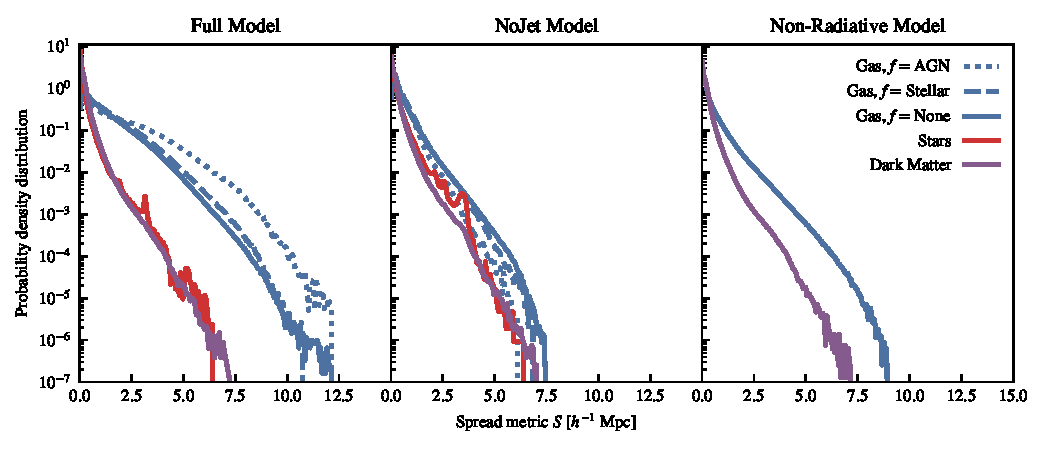
\includegraphics[width=\textwidth]{figures/neighbour_analysis_feedback_histogram_combined.pdf}
    \vspace{-0.7cm}
    \caption{Distribution of spread distances split by particle type for gas
    (blue), stars (red), and dark matter (purple). This is shown for the
    $z=0$ particle distribution in the reference model (left), the \nojet{}
    model (center), and the non-radiative simulation (right). The left and
    middle panels separate gas particles that have not been involved in any
    feedback event (solid) from those that have participated directly in
    either stellar (dashed) or AGN (dotted) feedback events. Jets are
    primarily responsible for spreading baryons to the largest distances in
    \simba{}, with significant entrainment of gas that did not directly
    participate in feedback events. The stellar distribution is significantly
    more noisy than the others due to the smaller number of star particles
    (compared to gas or dark matter) in the simulation.
    }\label{fig:feedbackdistance}
\end{figure*}

The kinetic feedback scheme used in \simba{} for both star formation and AGN
feedback makes it straightforward to identify the gas elements that have been
directly impacted by feedback. However, these gas elements will then go on to
entrain and deposit energy into other gas elements as they travel. This makes
it challenging to fully capture the impact of feedback solely from particle
tagging. Another option to assess feedback is to run simulations with
specific feedback modules turned on and off. However, this is inconsistent
with the tuning procedure that virtually every simulation suite performs in
order to constrain the many parameters in the sub-grid model. For instance,
modern models are typically calibrated to the $z=0$ Stellar Mass Function
(SMF), which will of course change should some energy injection mechanism be
missing (and hence the model should be re-calibrated). It is thus important
to realize that, if without some feedback module a simulation fails to match
data, this does not definitively prove that the feedback module is necessary
to produce realistic galaxies, since it could potentially be that the
simulation could be recalibrated to match data in some other way. In our
case, we run the \nojet{} and non-radiative variants in order to explore how
baryon redistribution is sensitive to these feedback modules, but we do not
attempt to recalibrate these to data, and merely use them in order to
investigate the impact of this input physics within the context of the
\simba{} model.

In Fig. \ref{fig:feedbackdistance}, we show different models in an attempt
to better characterise the effects of different pieces of the \simba{}
sub-grid model.

The left panel, showing the full \simba{} model, splits the gas component
into particles that have been affected by different types of feedback. Here,
AGN feedback takes precedence over stellar feedback, such that if a particle
has been affected by both it is only classified as being part of the $f=$AGN
group. We see that the particles that have directly interacted with the AGN
are spread to significantly larger distances, with a vertical offset of 0.5-1
dex compared to no-feedback particles for $S \gtrsim 5\hmpc{}$.
Particles that have been directly kicked by stellar feedback also have
systematically higher spread metric values, albeit with a smaller offset.
This implies that particles are indeed being spread to these large distances
by feedback events.

The left panel also now includes the stellar component, which shows a very
similar distribution to that of dark matter. It would be unexpected for a
star particle to form from a gas particle with a high spread value, as these
must have been separated dynamically from their closest dark matter
neighbour, requiring some kind of energy injection into the gas phase. This
would heat the particle, likely to a high temperature, making it less likely
that the particle will be able to cool by $z=0$ to a temperature low enough
to form a star. This then leaves the star to be affected by the same physics
that shape the spread distribution for the dark matter, namely tidal disruption,
stripping of satellites, and merger events.

The middle panel of Fig.~\ref{fig:feedbackdistance} shows the spread
distribution for the \nojet{} simulation, where we still include AGN feedback
in the form of radiative winds and X-ray heating but the high velocity jet
feedback mode is disabled. With this change, the spread metric is
significantly affected, with much less difference between the distributions
of the dark matter, gas, and stellar components. While galactic winds and AGN
feedback in radiative mode can still decouple the dark matter and gas
components, high-velocity jets are clearly the dominant mechanism responsible
for spreading baryons to the largest distances in \simba{}. Surprisingly, gas
particles directly kicked by feedback in this case show a lower spread
distribution compared to gas not directly impacted by feedback, in contrast
to the trend seen for the fiducial \simba{} model. This suggests that
feedback in the \nojet{} simulation is not strong enough to compensate for the
fact that feedback events occur in the densest regions (inside galaxies). It is
intrinsically more difficult to escape these deep potential wells, especially
now that a crucial energy injection mechanism from the AGN jets is missing.

This result is surprising given that less than $0.4\%$ of gas particles in
the simulation have ever interacted directly with the AGN jets; this has been
enough to significantly decouple the gas from the dark matter dynamically.
Such a high degree of separation points to substantial amounts of gas being
entrained by these powerful jets. It is not simply the case that higher mass
($M_H > 10^{11} \msolar{}$) haloes are quenched internally reducing their star
formation rate; the energetics and dynamics of the CGM and IGM are
significantly altered, as is already seen by the more complex interaction
between the turn-off of the galaxy stellar mass function (GSMF) and the power
of the AGN jets in many studies. 

The final contrast to highlight is the difference between the \nojet{} and
non-radiative model. The non-radiative model shows increased distance between
gas particles and their associated dark matter neighbour compared to the
\nojet{} run; this due to the lack of cooling preventing particles that lie
in small haloes from remaining as tightly bound. It also highlights how
difficult it is to drive gas into the centers of structures without cooling.
The collisionless dark matter can continue to fall in to bound structures,
with the gas being prevented due to strong accretion shocks. This allows for
a very different kind of separation than what we conjectured above about the
full physics models that include cooling.

\begin{figure}
    \centering
    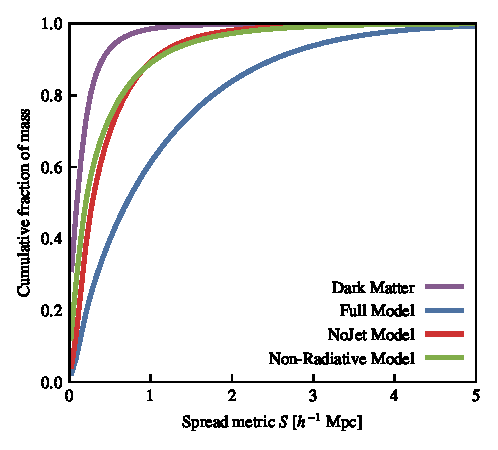
\includegraphics{figures/cumulative_histogram_comparison.pdf}
    \vspace{-0.7cm}
    \caption{Cumulative version of Fig. \ref{fig:feedbackdistance} that
    shows the gas distribution for the three models alongside the dark
    matter from the full model. This shows that 10\% of the
    gaseous matter has spread at least $3\hmpc{}$, with the same
    distance being only $0.5 \hmpc{}$ for the dark matter.}
    \label{fig:cumulativehistogram}
\end{figure}

In Fig. \ref{fig:cumulativehistogram} we show the cumulative version of Fig.
\ref{fig:feedbackdistance} to better show the amounts of mass that are spread
to large distances. The full model constrains about 90\% of the mass within
around $3\hmpc{}$, with a slow tail off ending with nearly all of the mass
being constrained to be spread less than $5\hmpc{}$.
